\chapter{Methodologies}
 In this chapter, I will be discussing the methodologies used in the project. Throughout the four years in GMIT, we were always told through several modules that software development methodologies and the choosing of the most suitable methodology for a given project were of extreme importance in any company that one would work in. Due to this, I researched different methodologies which I could use for my project, seeing the positives and negatives of each one. After researching each one I decided to go with using Agile as my main methodology. I felt this would be the best method to suit the development and it is also a widely used methodology in organizations around the world.

\section{Agile Development}
\begin{wrapfigure}{r}{0.25\textwidth} %this figure will be at the right
    \centering
    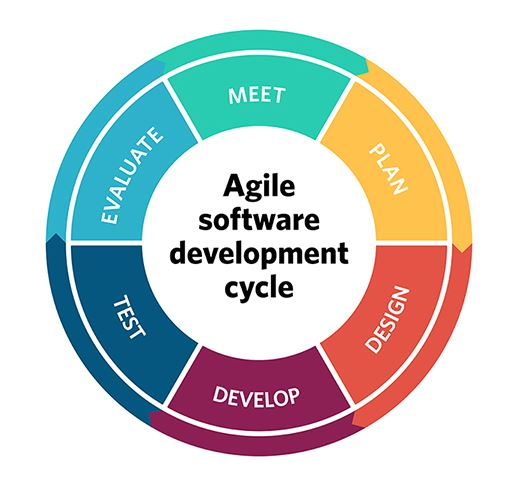
\includegraphics[width=0.3\textwidth]{Images/agile-software-development.jpg}
    \caption{Agile Cycle.}
  \label{fig:Agile Cycle}
\end{wrapfigure}
 Agile Development is a concept that allows that allows the product to be delivered to the customer in incremental releases as well as also being extremely flexible, which allows change to the requirements and allows the scope of the project to be increased without inflicting consequences on the design.

 The project contained Three main stages, research, design and implementation. For each stage I applied an agile like approach in order to complete them. I felt agile was best suited for the project as it allows for plenty of flexibility and allows the software to be delivered incrementally. I used a scrum like approach for each of the research, design and development processes. Scrum is an agile framework where members break their work into actions that are able to be completed within sprints, which are timed iterations, which usually last two weeks but can last up to a month long. Progress is then tracked and re-planned in meetings. \cite{AboutAgile}

\newpage

\subsection{Sprints}

A Sprint is a timed iteration of the continuous development cycle with a scrum being a discussion in the style of a meeting used to gain feedback. During the development of the project, my default sprint was a two week cycle after each meeting with my supervisor where I would plan what I would like to get done in the two week window. \cite{Sprints}

\begin{figure}[h]
  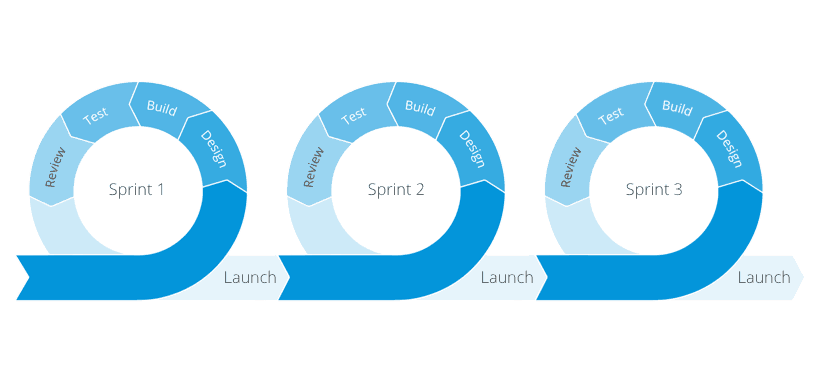
\includegraphics[width=\linewidth]{Images/AgileSprint.png}
  \caption{Sprint Cycle.}
  \label{fig:Sprint Cycle}
\end{figure}


\subsection{Meetings}

During the course of the college year, weekly meetings were held with a project supervisor to see how we were getting on with the project with initial meetings being used to brainstorm our ideas and get feedback on them. The meetings consisted of updates of our progress along with feedback on that progress, any advice or help was given to us if needed, and plans were put into place of what we would have done for the following meeting. If however a meeting could not be made, a simple email outlining what had been done and what was to be done next was sent to the supervisor to which they would promptly reply to giving their best advice and feedback.
\newpage

\section{Version Control}
\begin{figure}[h]
  
\includegraphics[width=\linewidth]{Images/GitHub.png}
  \caption{GitHub.}
  \label{fig:GitHub}
\end{figure}
For this project, I decided on using the online web-based GitHub Source Control Software. GitHub is a development platform which allows its users to use several collaboration features such as bug tracking in its issues section, task management, and a wiki for every project. These items were very useful when it came to the development of the project. GitHub is considered one of the most popular version control management services in the world and one we have used in the Software Development for the duration of the course for our project submissions. 
GitHub enabled me to be able to store both my dissertation and my project's repository. The main function allowed me to commit the work to repositories, allowing me to be able to get a previous  working version of the project. This was especially handy in case something happened where the project was broken and I couldn't fix it. This would allow me to clone the previously known working project and work again from that version. \cite{AboutGitHub}

\section{Technology Choice}
After researching Games development and what type of game I would be designing, I came to a conclusion as to what language I would be using and which game development software I would be using for the completion of my project. I decided on using the Unity game engine to develop my game and to use the C\# language to program the game. These choices were based on my previous experience in using both during the course of my 4 years in the Software Development course. Along with these I used Visual Studio Code and the image editor GIMP. Each of these technologies will be explained further in the Technology Review chapter.